\documentclass[1p]{elsarticle_modified}
%\bibliographystyle{elsarticle-num}

%\usepackage[colorlinks]{hyperref}
%\usepackage{abbrmath_seonhwa} %\Abb, \Ascr, \Acal ,\Abf, \Afrak
\usepackage{amsfonts}
\usepackage{amssymb}
\usepackage{amsmath}
\usepackage{amsthm}
\usepackage{scalefnt}
\usepackage{amsbsy}
\usepackage{kotex}
\usepackage{caption}
\usepackage{subfig}
\usepackage{color}
\usepackage{graphicx}
\usepackage{xcolor} %% white, black, red, green, blue, cyan, magenta, yellow
\usepackage{float}
\usepackage{setspace}
\usepackage{hyperref}

\usepackage{tikz}
\usetikzlibrary{arrows}

\usepackage{multirow}
\usepackage{array} % fixed length table
\usepackage{hhline}

%%%%%%%%%%%%%%%%%%%%%
\makeatletter
\renewcommand*\env@matrix[1][\arraystretch]{%
	\edef\arraystretch{#1}%
	\hskip -\arraycolsep
	\let\@ifnextchar\new@ifnextchar
	\array{*\c@MaxMatrixCols c}}
\makeatother %https://tex.stackexchange.com/questions/14071/how-can-i-increase-the-line-spacing-in-a-matrix
%%%%%%%%%%%%%%%

\usepackage[normalem]{ulem}

\newcommand{\msout}[1]{\ifmmode\text{\sout{\ensuremath{#1}}}\else\sout{#1}\fi}
%SOURCE: \msout is \stkout macro in https://tex.stackexchange.com/questions/20609/strikeout-in-math-mode

\newcommand{\cancel}[1]{
	\ifmmode
	{\color{red}\msout{#1}}
	\else
	{\color{red}\sout{#1}}
	\fi
}

\newcommand{\add}[1]{
	{\color{blue}\uwave{#1}}
}

\newcommand{\replace}[2]{
	\ifmmode
	{\color{red}\msout{#1}}{\color{blue}\uwave{#2}}
	\else
	{\color{red}\sout{#1}}{\color{blue}\uwave{#2}}
	\fi
}

\newcommand{\Sol}{\mathcal{S}} %segment
\newcommand{\D}{D} %diagram
\newcommand{\A}{\mathcal{A}} %arc


%%%%%%%%%%%%%%%%%%%%%%%%%%%%%5 test

\def\sl{\operatorname{\textup{SL}}(2,\Cbb)}
\def\psl{\operatorname{\textup{PSL}}(2,\Cbb)}
\def\quan{\mkern 1mu \triangleright \mkern 1mu}

\theoremstyle{definition}
\newtheorem{thm}{Theorem}[section]
\newtheorem{prop}[thm]{Proposition}
\newtheorem{lem}[thm]{Lemma}
\newtheorem{ques}[thm]{Question}
\newtheorem{cor}[thm]{Corollary}
\newtheorem{defn}[thm]{Definition}
\newtheorem{exam}[thm]{Example}
\newtheorem{rmk}[thm]{Remark}
\newtheorem{alg}[thm]{Algorithm}

\newcommand{\I}{\sqrt{-1}}
\begin{document}

%\begin{frontmatter}
%
%\title{Boundary parabolic representations of knots up to 8 crossings}
%
%%% Group authors per affiliation:
%\author{Yunhi Cho} 
%\address{Department of Mathematics, University of Seoul, Seoul, Korea}
%\ead{yhcho@uos.ac.kr}
%
%
%\author{Seonhwa Kim} %\fnref{s_kim}}
%\address{Center for Geometry and Physics, Institute for Basic Science, Pohang, 37673, Korea}
%\ead{ryeona17@ibs.re.kr}
%
%\author{Hyuk Kim}
%\address{Department of Mathematical Sciences, Seoul National University, Seoul 08826, Korea}
%\ead{hyukkim@snu.ac.kr}
%
%\author{Seokbeom Yoon}
%\address{Department of Mathematical Sciences, Seoul National University, Seoul, 08826,  Korea}
%\ead{sbyoon15@snu.ac.kr}
%
%\begin{abstract}
%We find all boundary parabolic representation of knots up to 8 crossings.
%
%\end{abstract}
%\begin{keyword}
%    \MSC[2010] 57M25 
%\end{keyword}
%
%\end{frontmatter}

%\linenumbers
%\tableofcontents
%
\newcommand\colored[1]{\textcolor{white}{\rule[-0.35ex]{0.8em}{1.4ex}}\kern-0.8em\color{red} #1}%
%\newcommand\colored[1]{\textcolor{white}{ #1}\kern-2.17ex	\textcolor{white}{ #1}\kern-1.81ex	\textcolor{white}{ #1}\kern-2.15ex\color{red}#1	}

{\Large $\underline{11a_{210}~(K11a_{210})}$}

\setlength{\tabcolsep}{10pt}
\renewcommand{\arraystretch}{1.6}
\vspace{1cm}\begin{tabular}{m{100pt}>{\centering\arraybackslash}m{274pt}}
\multirow{5}{120pt}{
	\centering
	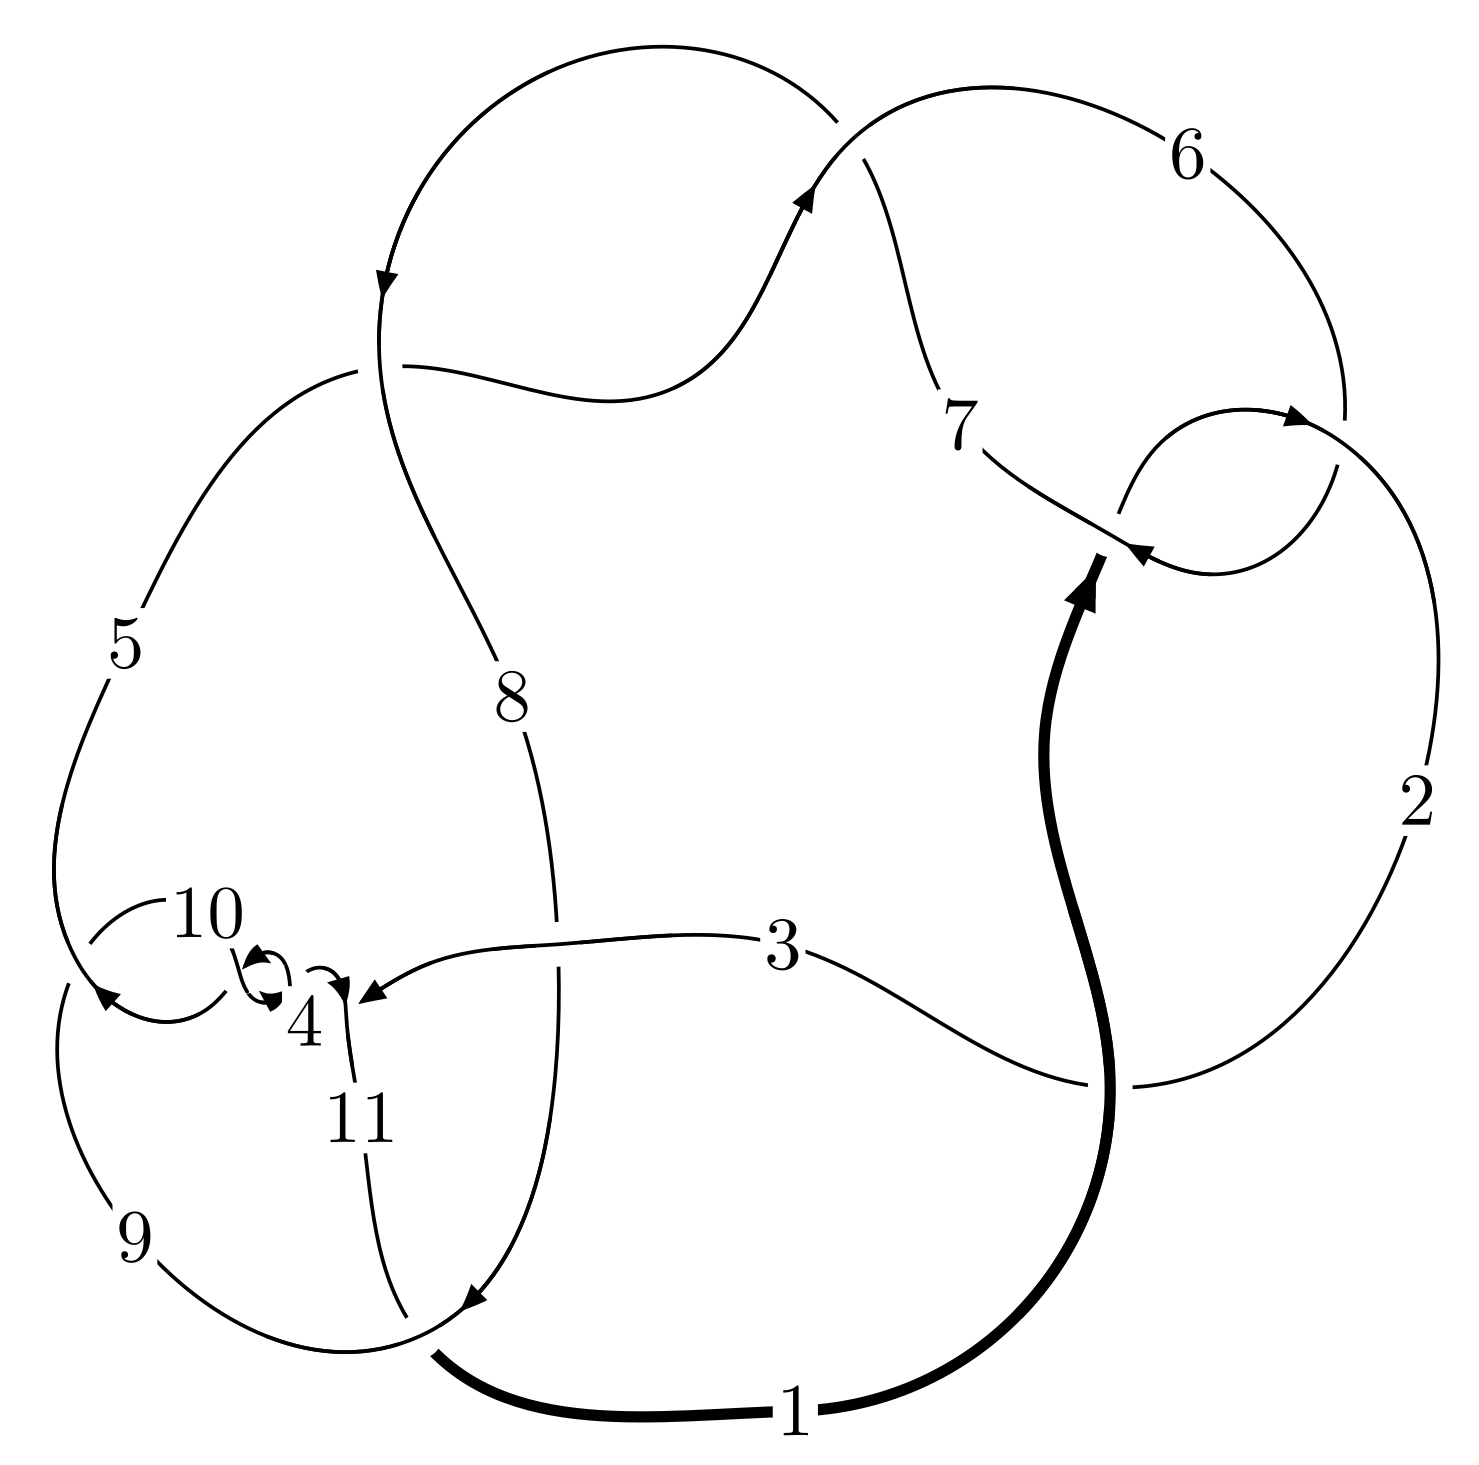
\includegraphics[width=112pt]{../../../GIT/diagram.site/Diagrams/png/459_11a_210.png}\\
\ \ \ A knot diagram\footnotemark}&
\allowdisplaybreaks
\textbf{Linearized knot diagam} \\
\cline{2-2}
 &
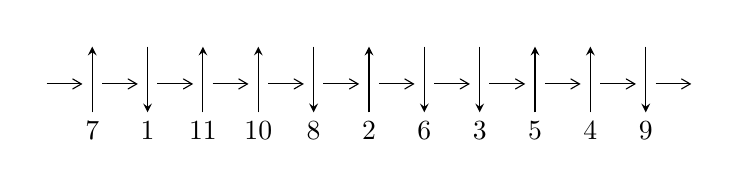
\begin{tikzpicture}[x=20pt, y=17pt]
	% nodes
	\node (C0) at (0, 0) {};
	\node (C1) at (1, 0) {};
	\node (C1U) at (1, +1) {};
	\node (C1D) at (1, -1) {7};

	\node (C2) at (2, 0) {};
	\node (C2U) at (2, +1) {};
	\node (C2D) at (2, -1) {1};

	\node (C3) at (3, 0) {};
	\node (C3U) at (3, +1) {};
	\node (C3D) at (3, -1) {11};

	\node (C4) at (4, 0) {};
	\node (C4U) at (4, +1) {};
	\node (C4D) at (4, -1) {10};

	\node (C5) at (5, 0) {};
	\node (C5U) at (5, +1) {};
	\node (C5D) at (5, -1) {8};

	\node (C6) at (6, 0) {};
	\node (C6U) at (6, +1) {};
	\node (C6D) at (6, -1) {2};

	\node (C7) at (7, 0) {};
	\node (C7U) at (7, +1) {};
	\node (C7D) at (7, -1) {6};

	\node (C8) at (8, 0) {};
	\node (C8U) at (8, +1) {};
	\node (C8D) at (8, -1) {3};

	\node (C9) at (9, 0) {};
	\node (C9U) at (9, +1) {};
	\node (C9D) at (9, -1) {5};

	\node (C10) at (10, 0) {};
	\node (C10U) at (10, +1) {};
	\node (C10D) at (10, -1) {4};

	\node (C11) at (11, 0) {};
	\node (C11U) at (11, +1) {};
	\node (C11D) at (11, -1) {9};
	\node (C12) at (12, 0) {};

	% arrows
	\draw[->,>={angle 60}]
	(C0) edge (C1) (C1) edge (C2) (C2) edge (C3) (C3) edge (C4) (C4) edge (C5) (C5) edge (C6) (C6) edge (C7) (C7) edge (C8) (C8) edge (C9) (C9) edge (C10) (C10) edge (C11) (C11) edge (C12) ;	\draw[->,>=stealth]
	(C1D) edge (C1U) (C2U) edge (C2D) (C3D) edge (C3U) (C4D) edge (C4U) (C5U) edge (C5D) (C6D) edge (C6U) (C7U) edge (C7D) (C8U) edge (C8D) (C9D) edge (C9U) (C10D) edge (C10U) (C11U) edge (C11D) ;
	\end{tikzpicture} \\
\hhline{~~} \\& 
\textbf{Solving Sequence} \\ \cline{2-2} 
 &
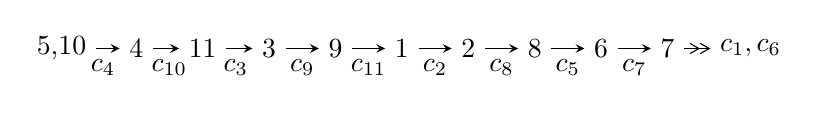
\begin{tikzpicture}[x=24pt, y=7pt]
	% node
	\node (A0) at (-1/8, 0) {5,10};
	\node (A1) at (1, 0) {4};
	\node (A2) at (2, 0) {11};
	\node (A3) at (3, 0) {3};
	\node (A4) at (4, 0) {9};
	\node (A5) at (5, 0) {1};
	\node (A6) at (6, 0) {2};
	\node (A7) at (7, 0) {8};
	\node (A8) at (8, 0) {6};
	\node (A9) at (9, 0) {7};
	\node (C1) at (1/2, -1) {$c_{4}$};
	\node (C2) at (3/2, -1) {$c_{10}$};
	\node (C3) at (5/2, -1) {$c_{3}$};
	\node (C4) at (7/2, -1) {$c_{9}$};
	\node (C5) at (9/2, -1) {$c_{11}$};
	\node (C6) at (11/2, -1) {$c_{2}$};
	\node (C7) at (13/2, -1) {$c_{8}$};
	\node (C8) at (15/2, -1) {$c_{5}$};
	\node (C9) at (17/2, -1) {$c_{7}$};
	\node (A10) at (41/4, 0) {$c_{1},c_{6}$};

	% edge
	\draw[->,>=stealth]	
	(A0) edge (A1) (A1) edge (A2) (A2) edge (A3) (A3) edge (A4) (A4) edge (A5) (A5) edge (A6) (A6) edge (A7) (A7) edge (A8) (A8) edge (A9) ;
	\draw[->>,>={angle 60}]	
	(A9) edge (A10);
\end{tikzpicture} \\ 

\end{tabular} \\

\footnotetext{
The image of knot diagram is generated by the software ``\textbf{Draw programme}" developed by Andrew Bartholomew(\url{http://www.layer8.co.uk/maths/draw/index.htm\#Running-draw}), where we modified some parts for our purpose(\url{https://github.com/CATsTAILs/LinksPainter}).
}\phantom \\ \newline 
\centering \textbf{Ideals for irreducible components\footnotemark of $X_{\text{par}}$} 
 
\begin{align*}
I^u_{1}&=\langle 
u^{36}- u^{35}+\cdots-2 u+1\rangle \\
\\
\end{align*}
\raggedright * 1 irreducible components of $\dim_{\mathbb{C}}=0$, with total 36 representations.\\
\footnotetext{All coefficients of polynomials are rational numbers. But the coefficients are sometimes approximated in decimal forms when there is not enough margin.}
\newpage
\renewcommand{\arraystretch}{1}
\centering \section*{I. $I^u_{1}= \langle u^{36}- u^{35}+\cdots-2 u+1 \rangle$}
\flushleft \textbf{(i) Arc colorings}\\
\begin{tabular}{m{7pt} m{180pt} m{7pt} m{180pt} }
\flushright $a_{5}=$&$\begin{pmatrix}1\\0\end{pmatrix}$ \\
\flushright $a_{10}=$&$\begin{pmatrix}0\\u\end{pmatrix}$ \\
\flushright $a_{4}=$&$\begin{pmatrix}1\\u^2\end{pmatrix}$ \\
\flushright $a_{11}=$&$\begin{pmatrix}u\\u^3+u\end{pmatrix}$ \\
\flushright $a_{3}=$&$\begin{pmatrix}u^2+1\\u^4+2 u^2\end{pmatrix}$ \\
\flushright $a_{9}=$&$\begin{pmatrix}- u\\u\end{pmatrix}$ \\
\flushright $a_{1}=$&$\begin{pmatrix}- u^5-2 u^3+u\\u^5+3 u^3+u\end{pmatrix}$ \\
\flushright $a_{2}=$&$\begin{pmatrix}u^{14}+7 u^{12}+16 u^{10}+11 u^8-2 u^6+1\\- u^{14}-8 u^{12}-23 u^{10}-28 u^8-14 u^6-4 u^4+u^2\end{pmatrix}$ \\
\flushright $a_{8}=$&$\begin{pmatrix}u^7+4 u^5+4 u^3\\u^9+5 u^7+7 u^5+2 u^3+u\end{pmatrix}$ \\
\flushright $a_{6}=$&$\begin{pmatrix}u^{16}+9 u^{14}+31 u^{12}+50 u^{10}+37 u^8+12 u^6+4 u^4+1\\u^{18}+10 u^{16}+39 u^{14}+74 u^{12}+71 u^{10}+38 u^8+18 u^6+4 u^4+u^2\end{pmatrix}$ \\
\flushright $a_{7}=$&$\begin{pmatrix}u^{25}+14 u^{23}+\cdots+6 u^3+u\\u^{27}+15 u^{25}+\cdots+3 u^3+u\end{pmatrix}$\\ \flushright $a_{7}=$&$\begin{pmatrix}u^{25}+14 u^{23}+\cdots+6 u^3+u\\u^{27}+15 u^{25}+\cdots+3 u^3+u\end{pmatrix}$\\&\end{tabular}
\flushleft \textbf{(ii) Obstruction class $= -1$}\\~\\
\flushleft \textbf{(iii) Cusp Shapes $= -4 u^{34}+4 u^{33}-80 u^{32}+76 u^{31}-712 u^{30}+640 u^{29}-3712 u^{28}+3144 u^{27}-12568 u^{26}+9996 u^{25}-29012 u^{24}+21652 u^{23}-46856 u^{22}+33008 u^{21}-53996 u^{20}+36580 u^{19}-45668 u^{18}+30752 u^{17}-29624 u^{16}+20396 u^{15}-15384 u^{14}+10740 u^{13}-6764 u^{12}+4600 u^{11}-2980 u^{10}+1824 u^9-1312 u^8+688 u^7-460 u^6+268 u^5-128 u^4+92 u^3-20 u^2+12 u-6$}\\~\\
\newpage\renewcommand{\arraystretch}{1}
\flushleft \textbf{(iv) u-Polynomials at the component}\newline \\
\begin{tabular}{m{50pt}|m{274pt}}
Crossings & \hspace{64pt}u-Polynomials at each crossing \\
\hline $$\begin{aligned}c_{1},c_{6}\end{aligned}$$&$\begin{aligned}
&u^{36}+u^{35}+\cdots+u^2+1
\end{aligned}$\\
\hline $$\begin{aligned}c_{2},c_{5},c_{7}\end{aligned}$$&$\begin{aligned}
&u^{36}+9 u^{35}+\cdots+2 u+1
\end{aligned}$\\
\hline $$\begin{aligned}c_{3},c_{4},c_{9}\\c_{10}\end{aligned}$$&$\begin{aligned}
&u^{36}+u^{35}+\cdots+2 u+1
\end{aligned}$\\
\hline $$\begin{aligned}c_{8}\end{aligned}$$&$\begin{aligned}
&u^{36}+u^{35}+\cdots+24 u+5
\end{aligned}$\\
\hline $$\begin{aligned}c_{11}\end{aligned}$$&$\begin{aligned}
&u^{36}-9 u^{35}+\cdots+8 u+1
\end{aligned}$\\
\hline
\end{tabular}\\~\\
\newpage\renewcommand{\arraystretch}{1}
\flushleft \textbf{(v) Riley Polynomials at the component}\newline \\
\begin{tabular}{m{50pt}|m{274pt}}
Crossings & \hspace{64pt}Riley Polynomials at each crossing \\
\hline $$\begin{aligned}c_{1},c_{6}\end{aligned}$$&$\begin{aligned}
&y^{36}+9 y^{35}+\cdots+2 y+1
\end{aligned}$\\
\hline $$\begin{aligned}c_{2},c_{5},c_{7}\end{aligned}$$&$\begin{aligned}
&y^{36}+37 y^{35}+\cdots+18 y+1
\end{aligned}$\\
\hline $$\begin{aligned}c_{3},c_{4},c_{9}\\c_{10}\end{aligned}$$&$\begin{aligned}
&y^{36}+41 y^{35}+\cdots+2 y+1
\end{aligned}$\\
\hline $$\begin{aligned}c_{8}\end{aligned}$$&$\begin{aligned}
&y^{36}-3 y^{35}+\cdots-6 y+25
\end{aligned}$\\
\hline $$\begin{aligned}c_{11}\end{aligned}$$&$\begin{aligned}
&y^{36}+y^{35}+\cdots-30 y+1
\end{aligned}$\\
\hline
\end{tabular}\\~\\
\newpage\flushleft \textbf{(vi) Complex Volumes and Cusp Shapes}
$$\begin{array}{c|c|c}  
\text{Solutions to }I^u_{1}& \I (\text{vol} + \sqrt{-1}CS) & \text{Cusp shape}\\
 \hline 
\begin{aligned}
u &= \phantom{-}0.039758 + 0.866938 I\end{aligned}
 & \phantom{-}2.43227 - 2.98822 I & -1.17573 + 2.50595 I \\ \hline\begin{aligned}
u &= \phantom{-}0.039758 - 0.866938 I\end{aligned}
 & \phantom{-}2.43227 + 2.98822 I & -1.17573 - 2.50595 I \\ \hline\begin{aligned}
u &= \phantom{-}0.528849 + 0.662164 I\end{aligned}
 & \phantom{-}5.28964 + 8.99184 I & \phantom{-}2.24371 - 8.34910 I \\ \hline\begin{aligned}
u &= \phantom{-}0.528849 - 0.662164 I\end{aligned}
 & \phantom{-}5.28964 - 8.99184 I & \phantom{-}2.24371 + 8.34910 I \\ \hline\begin{aligned}
u &= -0.529498 + 0.643326 I\end{aligned}
 & \phantom{-}5.68597 - 2.74218 I & \phantom{-}3.17354 + 3.44962 I \\ \hline\begin{aligned}
u &= -0.529498 - 0.643326 I\end{aligned}
 & \phantom{-}5.68597 + 2.74218 I & \phantom{-}3.17354 - 3.44962 I \\ \hline\begin{aligned}
u &= \phantom{-}0.434530 + 0.674620 I\end{aligned}
 & -2.03776 + 5.19435 I & -3.33716 - 9.21025 I \\ \hline\begin{aligned}
u &= \phantom{-}0.434530 - 0.674620 I\end{aligned}
 & -2.03776 - 5.19435 I & -3.33716 + 9.21025 I \\ \hline\begin{aligned}
u &= \phantom{-}0.279015 + 0.697032 I\end{aligned}
 & -3.00780 + 0.17019 I & -7.29367 - 0.75206 I \\ \hline\begin{aligned}
u &= \phantom{-}0.279015 - 0.697032 I\end{aligned}
 & -3.00780 - 0.17019 I & -7.29367 + 0.75206 I \\ \hline\begin{aligned}
u &= -0.401351 + 0.583059 I\end{aligned}
 & \phantom{-}0.07417 - 1.89235 I & \phantom{-}3.15479 + 4.52320 I \\ \hline\begin{aligned}
u &= -0.401351 - 0.583059 I\end{aligned}
 & \phantom{-}0.07417 + 1.89235 I & \phantom{-}3.15479 - 4.52320 I \\ \hline\begin{aligned}
u &= -0.588252 + 0.276624 I\end{aligned}
 & \phantom{-}6.75859 - 1.08065 I & \phantom{-}5.91547 + 2.62482 I \\ \hline\begin{aligned}
u &= -0.588252 - 0.276624 I\end{aligned}
 & \phantom{-}6.75859 + 1.08065 I & \phantom{-}5.91547 - 2.62482 I \\ \hline\begin{aligned}
u &= \phantom{-}0.596249 + 0.252176 I\end{aligned}
 & \phantom{-}6.48998 - 5.15115 I & \phantom{-}5.34177 + 2.63886 I \\ \hline\begin{aligned}
u &= \phantom{-}0.596249 - 0.252176 I\end{aligned}
 & \phantom{-}6.48998 + 5.15115 I & \phantom{-}5.34177 - 2.63886 I \\ \hline\begin{aligned}
u &= -0.014393 + 1.396600 I\end{aligned}
 & \phantom{-}1.85163 - 3.15004 I & \phantom{-0.000000 -}0. + 2.61659 I \\ \hline\begin{aligned}
u &= -0.014393 - 1.396600 I\end{aligned}
 & \phantom{-}1.85163 + 3.15004 I & \phantom{-0.000000 } 0. - 2.61659 I \\ \hline\begin{aligned}
u &= -0.383996 + 0.360002 I\end{aligned}
 & \phantom{-}0.721812 - 0.963189 I & \phantom{-}5.72873 + 5.37633 I \\ \hline\begin{aligned}
u &= -0.383996 - 0.360002 I\end{aligned}
 & \phantom{-}0.721812 + 0.963189 I & \phantom{-}5.72873 - 5.37633 I \\ \hline\begin{aligned}
u &= \phantom{-}0.469156 + 0.145748 I\end{aligned}
 & -0.55346 - 2.03006 I & \phantom{-}1.12004 + 4.04451 I \\ \hline\begin{aligned}
u &= \phantom{-}0.469156 - 0.145748 I\end{aligned}
 & -0.55346 + 2.03006 I & \phantom{-}1.12004 - 4.04451 I \\ \hline\begin{aligned}
u &= -0.04789 + 1.52934 I\end{aligned}
 & -5.61681 - 2.13861 I & \phantom{-0.000000 } 0 \\ \hline\begin{aligned}
u &= -0.04789 - 1.52934 I\end{aligned}
 & -5.61681 + 2.13861 I & \phantom{-0.000000 } 0 \\ \hline\begin{aligned}
u &= -0.11001 + 1.57378 I\end{aligned}
 & -7.26818 - 3.72706 I & \phantom{-0.000000 } 0 \\ \hline\begin{aligned}
u &= -0.11001 - 1.57378 I\end{aligned}
 & -7.26818 + 3.72706 I & \phantom{-0.000000 } 0 \\ \hline\begin{aligned}
u &= -0.15462 + 1.58238 I\end{aligned}
 & -1.80521 - 5.25682 I & \phantom{-0.000000 } 0 \\ \hline\begin{aligned}
u &= -0.15462 - 1.58238 I\end{aligned}
 & -1.80521 + 5.25682 I & \phantom{-0.000000 } 0 \\ \hline\begin{aligned}
u &= \phantom{-}0.15565 + 1.58986 I\end{aligned}
 & -2.30348 + 11.52240 I & \phantom{-0.000000 } 0 \\ \hline\begin{aligned}
u &= \phantom{-}0.15565 - 1.58986 I\end{aligned}
 & -2.30348 - 11.52240 I & \phantom{-0.000000 } 0\\
 \hline 
 \end{array}$$\newpage$$\begin{array}{c|c|c}  
\text{Solutions to }I^u_{1}& \I (\text{vol} + \sqrt{-1}CS) & \text{Cusp shape}\\
 \hline 
\begin{aligned}
u &= \phantom{-}0.08438 + 1.59811 I\end{aligned}
 & -10.84150 + 1.55360 I & \phantom{-0.000000 } 0 \\ \hline\begin{aligned}
u &= \phantom{-}0.08438 - 1.59811 I\end{aligned}
 & -10.84150 - 1.55360 I & \phantom{-0.000000 } 0 \\ \hline\begin{aligned}
u &= \phantom{-}0.12378 + 1.59576 I\end{aligned}
 & -9.75368 + 7.25706 I & \phantom{-0.000000 } 0 \\ \hline\begin{aligned}
u &= \phantom{-}0.12378 - 1.59576 I\end{aligned}
 & -9.75368 - 7.25706 I & \phantom{-0.000000 } 0 \\ \hline\begin{aligned}
u &= \phantom{-}0.01864 + 1.60315 I\end{aligned}
 & -5.85535 - 2.75781 I & \phantom{-0.000000 } 0 \\ \hline\begin{aligned}
u &= \phantom{-}0.01864 - 1.60315 I\end{aligned}
 & -5.85535 + 2.75781 I & \phantom{-0.000000 } 0\\
 \hline 
 \end{array}$$\newpage
\newpage\renewcommand{\arraystretch}{1}
\centering \section*{ II. u-Polynomials}
\begin{tabular}{m{50pt}|m{274pt}}
Crossings & \hspace{64pt}u-Polynomials at each crossing \\
\hline $$\begin{aligned}c_{1},c_{6}\end{aligned}$$&$\begin{aligned}
&u^{36}+u^{35}+\cdots+u^2+1
\end{aligned}$\\
\hline $$\begin{aligned}c_{2},c_{5},c_{7}\end{aligned}$$&$\begin{aligned}
&u^{36}+9 u^{35}+\cdots+2 u+1
\end{aligned}$\\
\hline $$\begin{aligned}c_{3},c_{4},c_{9}\\c_{10}\end{aligned}$$&$\begin{aligned}
&u^{36}+u^{35}+\cdots+2 u+1
\end{aligned}$\\
\hline $$\begin{aligned}c_{8}\end{aligned}$$&$\begin{aligned}
&u^{36}+u^{35}+\cdots+24 u+5
\end{aligned}$\\
\hline $$\begin{aligned}c_{11}\end{aligned}$$&$\begin{aligned}
&u^{36}-9 u^{35}+\cdots+8 u+1
\end{aligned}$\\
\hline
\end{tabular}\newpage\renewcommand{\arraystretch}{1}
\centering \section*{ III. Riley Polynomials}
\begin{tabular}{m{50pt}|m{274pt}}
Crossings & \hspace{64pt}Riley Polynomials at each crossing \\
\hline $$\begin{aligned}c_{1},c_{6}\end{aligned}$$&$\begin{aligned}
&y^{36}+9 y^{35}+\cdots+2 y+1
\end{aligned}$\\
\hline $$\begin{aligned}c_{2},c_{5},c_{7}\end{aligned}$$&$\begin{aligned}
&y^{36}+37 y^{35}+\cdots+18 y+1
\end{aligned}$\\
\hline $$\begin{aligned}c_{3},c_{4},c_{9}\\c_{10}\end{aligned}$$&$\begin{aligned}
&y^{36}+41 y^{35}+\cdots+2 y+1
\end{aligned}$\\
\hline $$\begin{aligned}c_{8}\end{aligned}$$&$\begin{aligned}
&y^{36}-3 y^{35}+\cdots-6 y+25
\end{aligned}$\\
\hline $$\begin{aligned}c_{11}\end{aligned}$$&$\begin{aligned}
&y^{36}+y^{35}+\cdots-30 y+1
\end{aligned}$\\
\hline
\end{tabular}
\vskip 2pc
\end{document}